\chapter{Craindre des dérives ou se réjouir des bénéfices ?}

\section{Légaliser : vers un abus de la Beuh ?}

Tout comme pour de nombreuses substances nocives ou potentiellement nocives pour l’homme (alcool, café etc), le principal objectif du débat sur le cannabis est d’en réduire sa consommation parmi la population. Actuellement en France le cannabis est illégal, il est donc normal de se demander si sa légalisation n’entrainerait pas un abus de la beuh ; si autoriser l’interdit n’entraîne-t-il pas une hausse de sa consommation ?

\paragraph{Des similarités avec le cas de l'alcool ?}

 	Pour commencer, selon un rapport de l’ECDE (Organisation de coopération et de développement économiques) de mai 2015 sur les pratiques de \textit{binge drinking} (beuveries express) chez les jeunes \cite{oecd}, la facilité d’accès à l’alcool est une des raisons majeures de l’apparition et de la popularisation des dérives sur sa consommation. En effet ce rapport nous apprend par exemple que la part des garçons qui, à 15 ans, n’ont jamais bu d’alcool est passée de 44\% en 2001-02 à 30\% en 2009-10. La proportion de ceux qui à 15 ans ont déjà été ivres au moins une fois, est passée de 30\% à 43\% sur la même période. Des effets similaires sont présent chez les jeunes filles et avec cela des pratiques telle que le \textit{binge drinking} sont en augmentation. D’un autre côté, un rapport de l’IRDES (Institut de recherche et de documentation en économie de la santé) nous dit qu’en 2013, les ivresses chez les jeunes sont « plus fréquentes qu’en 2001 mais moins qu’en 1996 » \cite{irdes}. Nous voyons donc qu’il existe un possible « effet de mode générationnel » lui-même responsable dans les abus de consommation d’alcool mais il est évident que l’accessibilité de l’alcool seule est une source de dérives ; cela ne va-t-il pas être de même pour le cannabis ? 
    
    Globalement comme nous l’avons vu, le nombre de consommateurs réguliers de marijuana post-légalisation va dépendre du système dans lequel cette légalisation va être mise en place. Dans le scénario que nous trouvons comme étant le plus adapté, celui d’un monopole géré par l’État, ce nombre va probablement rester le même. En effet actuellement le cannabis est considéré comme étant très accessible pour un produit illégal : pour preuves le nombre important de consommateurs en France; son prix ---~fin 2014, le gramme de cannabis est en moyenne estimé à 6~\euro\ en France \cite{terraNova_rapport}; et l’avis de la population ---~en 2011, 43\% des adolescents français de 15-16 ans estimaient que, s’ils le voulaient, il leur serait « facile » d’obtenir du cannabis \cite{obradovic15}. \textit{Sa légalisation ne le rendrait donc pas beaucoup plus facilement atteignable}, et n’amènerait pas à un abus de sa consommation. 

\paragraph{Effet de mode/effet Streisand}

Nous pouvons ensuite également nous demander si cette légalisation ne créerait pas un effet de mode sur la marijuana. Cependant si « buzz » il y a, il ne serait que de courte durée et ne produirait une augmentation significative que du nombre de personne ayant testé au moins une fois le cannabis. À part cela, il n’existe pas de raisons pour que la légalisation rende la marijuana attractive sur le long terme. Au contraire, en étant illégal, le cannabis souffre d’un « effet Streisand » ---~ce qui est interdit attire~---, qui par définition est voué à disparaître en cas de légalisation. Pour expliquer ce phénomène d’effet Streisand, nous pouvons reprendre l’exemple de l’alcool : la prohibition de l’alcool aux Etats-Unis de 1919 à 1933 nous permet de montrer que l’interdiction d’une substance récréative entraîne de nombreux problèmes. À cette époque, cette politique divise les États-Unis entre « secs » et « mouillés » et entraîne une perte de revenus et création de dépenses pour l’État. Un immense marché noir se met en place,  provoquant l'arrivée de boissons nocives sur le marché, l'augmentation des prix de l’alcool et celle de la corruption. Étonnamment, \textit{l’interdiction eu la conséquence perverse d’augmenter la consommation d’alcool} sur le territoire américain \cite{prohibition20} : c'est ce qu'on appelle l'effet Streisand.

On peut tracer un parallèle avec le cannabis : en cas de légalisation, le cannabis se retrouverait au même niveau que des substances comme l’alcool ou le tabac aujourd’hui en France. 


\paragraph{Et chez les autres, comment cela s'est-il passé ?}

Afin d’appuyer ce que nous venons de dire, nous pouvons nous pencher sur des pays moins fermes vis-à-vis du cannabis. Nous allons prendre l’exemple des États-Unis, dont plusieurs États ont légalisé le chanvre, puis nous verrons le cas des pays Européens, et notamment celui des Pays-Bas.

\paragraph{L'Uruguay, un bilan à nuancer}

Nous n’allons pas cependant nous intéresser au cas de l’Uruguay même si celui-ci est le premier pays à avoir voté une loi visant à réguler la chaîne de production de marijuana nationale. Premièrement, le niveau de vie du pays et sa culture sont bien trop différents des nôtres : son PIB est 45 fois plus bas que celui de la France (source Banque mondiale). De plus la plupart des résultats sortant de ce projet qualifié « d’expérience sociale » par l’ex-président Jose Mujica sont assez peu exploitables. Par exemple, le nombre de consommateurs de marijuana chez les jeunes entre treize et dix-sept ans est utilisé par les prohibitionnistes comme argument contre la légalisation du cannabis. De leur côté, les pro-cannabis réfutent cet argument, le considérant comme faisant partie d’une tendance générale, le nombre de consommateur ayant commencé son augmentation bien avant la loi du 6 mai 2015. 

Il est donc difficile d'utiliser les résultats de cette « expérience », cependant l’Uruguay a permis de montrer de manière irréfutable les difficultés, pour un pays manquant de moyens, à lutter contre le narcotrafic grâce à la légalisation. En causes : les difficultés à fournir des quantités suffisantes de cannabis aux pharmacies et autres distributeurs, les difficultés à rivaliser avec les tarifs du marché noir et enfin la défiance du peuple vis-à-vis des intentions de l’État \fullcite{uruguaybilan}.

\paragraph{Les États-unis sur la voie de la légalisation }

Premièrement donc en regardant ce qu’il se passe aux États-Unis, nous pouvons voir que dans les états comme l’Oregon ou le Colorado, où le cannabis est aujourd’hui légal, la légalisation de la plante n’a pas eu d’effet notable sur le nombre de jeunes consommateurs. De plus, la légalisation du cannabis ---~considéré par beaucoup comme une drogue d’introduction~---, n’a pas eu non plus d’effets sur la consommation d’autres drogues \cite{reality}. En revanche, malgré ces dires, certains chiffres et graphiques peuvent laisser le doute sur le manque d’impact négatif de la légalisation sur l’augmentation de la consommation de cannabis. 

\begin{figure}\centering
	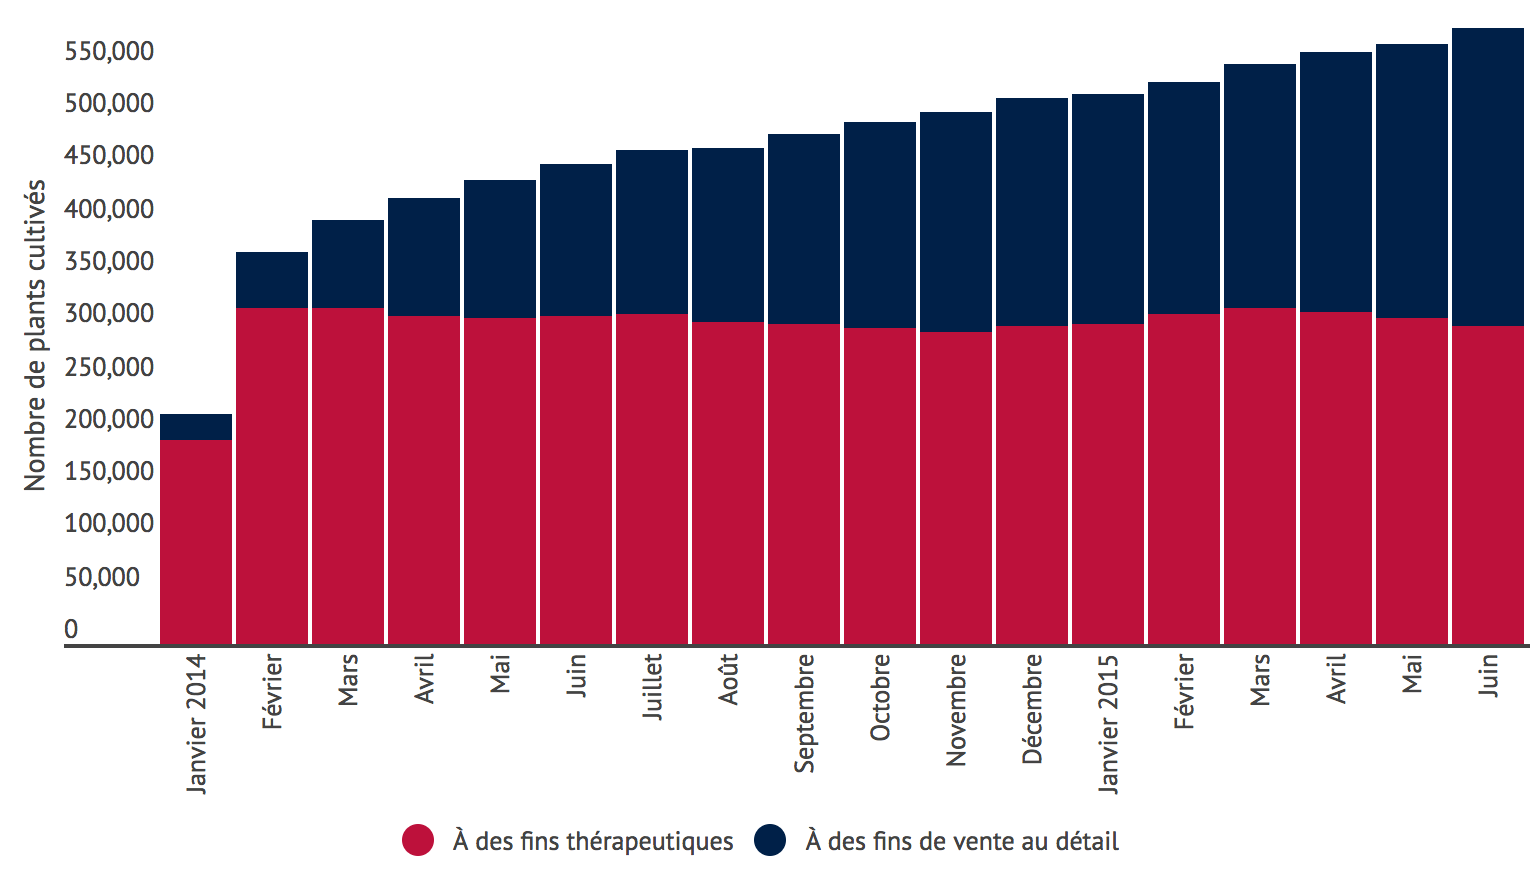
\includegraphics[width=\textwidth]{images/grapheconso.png}
    \caption{Nombre de plants cultivés au Colorado depuis la légalisation en 2014}
    \label{fig:grapheconso}
\end{figure}


Par exemple sur le graphique \ref{fig:grapheconso}, nous voyons qu’au Colorado, depuis la légalisation, le nombre de plants cultivés ne cesse d’augmenter. Cependant il faut rester sur ses gardes avec ces chiffres, il est en effet logique que ce chiffre croisse, le marché du cannabis se mettant en place avec sa concurrence sans vouloir indiquer une augmentation de la consommation de cannabis. En conclusion, pour le moment, la légalisation du cannabis aux États-Unis est plutôt considérée comme étant une réussite.

\paragraph{Depuis 1976, les Pays-Bas ont une politique dite de tolérance dans ce domaine :}

\begin{figure}\centering
	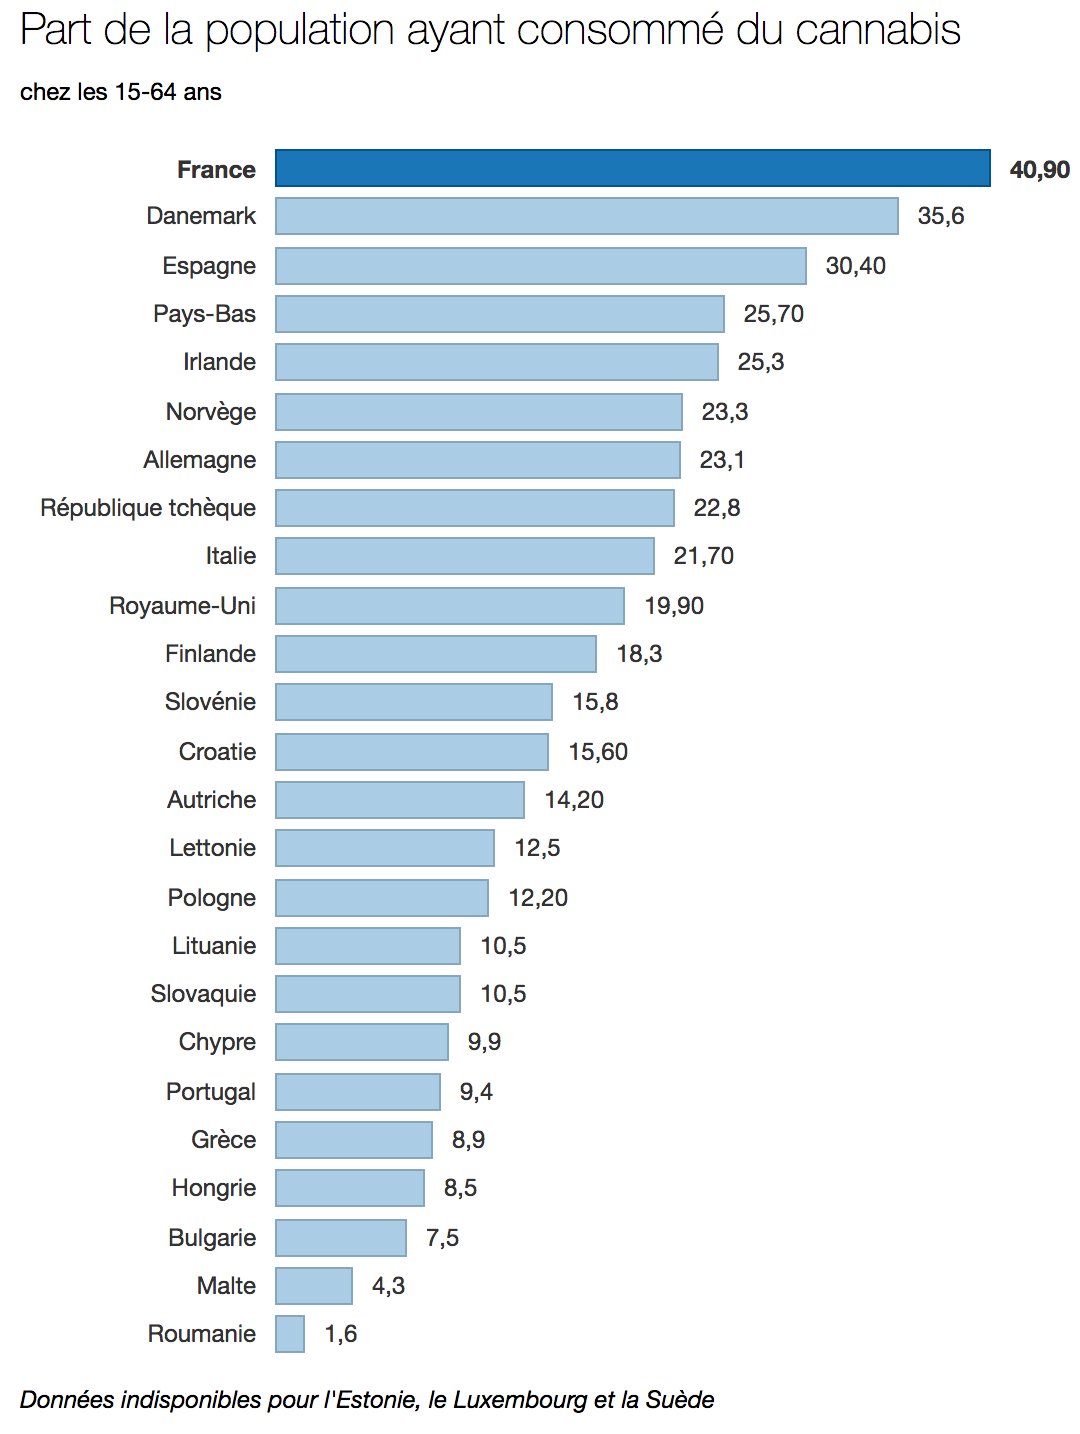
\includegraphics[height=.4\textheight]{images/grapheconsoPop.png}
    \caption{Part de la population ayant consommé du cannabis dans différents pays d'Europe}
    \label{fig:grapheconsopop}
\end{figure}

Enfin, un dernier élément va nous permettre de montrer que légaliser le cannabis peut permettre d’en éviter les abus. En effet, alors que la France est une des pays européens les plus répressif sur la question du haschich, nous voyons sur la figure \ref{fig:grapheconsopop} qu’elle est pourtant plus grande consommatrice que ses voisins. Comment expliquer qu’aux Pays-Bas, où le cannabis baigne dans une politique dite de tolérance depuis 1976, il y ait si « peu » de consommateurs ? Certes on dit que la pelouse est toujours plus verte chez notre voisin mais on peut quand même s'interroger sérieusement. Plusieurs raisons simples expliquent cela. Tout d’abord, le cannabis une fois autorisé est moins repoussant, moins tabou, il est donc plus facile d’éduquer la population sur le sujet et dès l’école. De plus, avec les revenus de la légalisation, il est possible d’être plus efficace sur la prévention, le système de santé, l’éducation etc. \cite{drugreport}

\section{Le cannabis, une bomb pour la santé ?}

Après avoir vu comment la légalisation du cannabis pouvait en influencer sa consommation, nous allons maintenant nous intéresser à la question de la santé. Une première interrogation se pose : est-il raisonnable de légaliser une substance qui peut affecter la santé ? Bien entendu, la réponse est non, en tous cas cela n’est pas plus raisonnable que de laisser légal et accessible de nombreuses autres drogues présente sur le marché qui ont, contrairement au cannabis bien plus la main rouge que la main verte.

\paragraph{Comparaison à des drogues légales}

En effet lorsque l’on regarde le bilan meurtrier de quelques substances qui nous sont bien familières, on se rend vite compte que le cannabis est en comparaison assez inoffensif. Dans le film-documentaire « The Union : the business behind getting high » de Brett Harvey, on apprend qu’en 2007 (année de sortie du film), aux États-Unis, les cachets de type aspirine ont provoqué la mort de 7500 personnes, le bilan du café s’élève lui à 10 000 victimes, vient ensuite l’alcool, responsable de  85 000 décès et enfin loin devant, nous retrouvons le tabac, meurtrier d’environ 450 000 personnes. C’est plus que les décès causés par le Sida, le crack, l’héroïne, les accidents de voiture, les meurtres, les incendies et l’alcool réunis. D’un autre côté, le docteur Lester Grinspoon nous apprend que depuis sa première utilisation par l’Homme, le cannabis n’a été relié à aucun décès (si l’on s’intéresse aux morts dûes à la substance seule). En effet il est pratiquement impossible pour l’Homme de faire une overdose suite à la consommation de marijuana, selon le docteur Paul Hornby, il faudrait fumer l’équivalent de 15 000 joints en à peine plus de 10 minutes pour risquer l’overdose. Ces chiffres son cependant à revoir à la baisse aujourd’hui, étant donné l’augmentation constante de la teneur en THC de la plante sur le marché noir. 

\paragraph{Les risques du cannabis :}

Vient ensuite la question du cancer, en effet la principale méthode de consommation du cannabis se fait par l’inhalation de fumée, cette méthode n’est-elle pas à risque ? Malheureusement, pour cette question, il nous est compliqué d’apporter une réponse, les études à ce sujet se contredisant énormément. Certaines nous disent que la fumée de cannabis contient dans une large mesure les mêmes substances cancérigènes que le tabac parfois en concentration plus forte, qu’en fumant du cannabis, on absorbe plus de monoxyde de carbone qu’en fumant du tabac, ou bien que le cannabinoïde méthandamide synthétique intensifie le développement des cellules du cancer du poumon et que la vaporisation prévient le dégagement de goudron et d’autres substances nocives et cancérogènes ---~c’est pourquoi il s’agit d’un des rares modes d’administration validé médicalement.\cite{cannacancer} 

Parallèlement, certaines publications scientifiques révèlent tout l’inverse, le cannabis n’aurait pas de lien avec le cancer de poumon, au contraire, l’inhalation de THC permettrait d’éliminer les potentielles cellules cancéreuses et donc de lutter contre le cancer. \cite{washington} Dans le film de Brett Harvey, le seul fait que de telles controverses existent est utilisé pour défendre le cannabis : « Si le cannabis avait un réel lien avec le déclenchement de cancer, ce dernier aurait été découvert depuis longtemps ».

Pour résumer le danger du cannabis en comparaison avec d’autres drogues nous pouvons utiliser les résultats du rapport sur la dangerosité des produits par le professeur Bernard Roques (table \ref{tab:drogues}).

\begin{table}\centering
	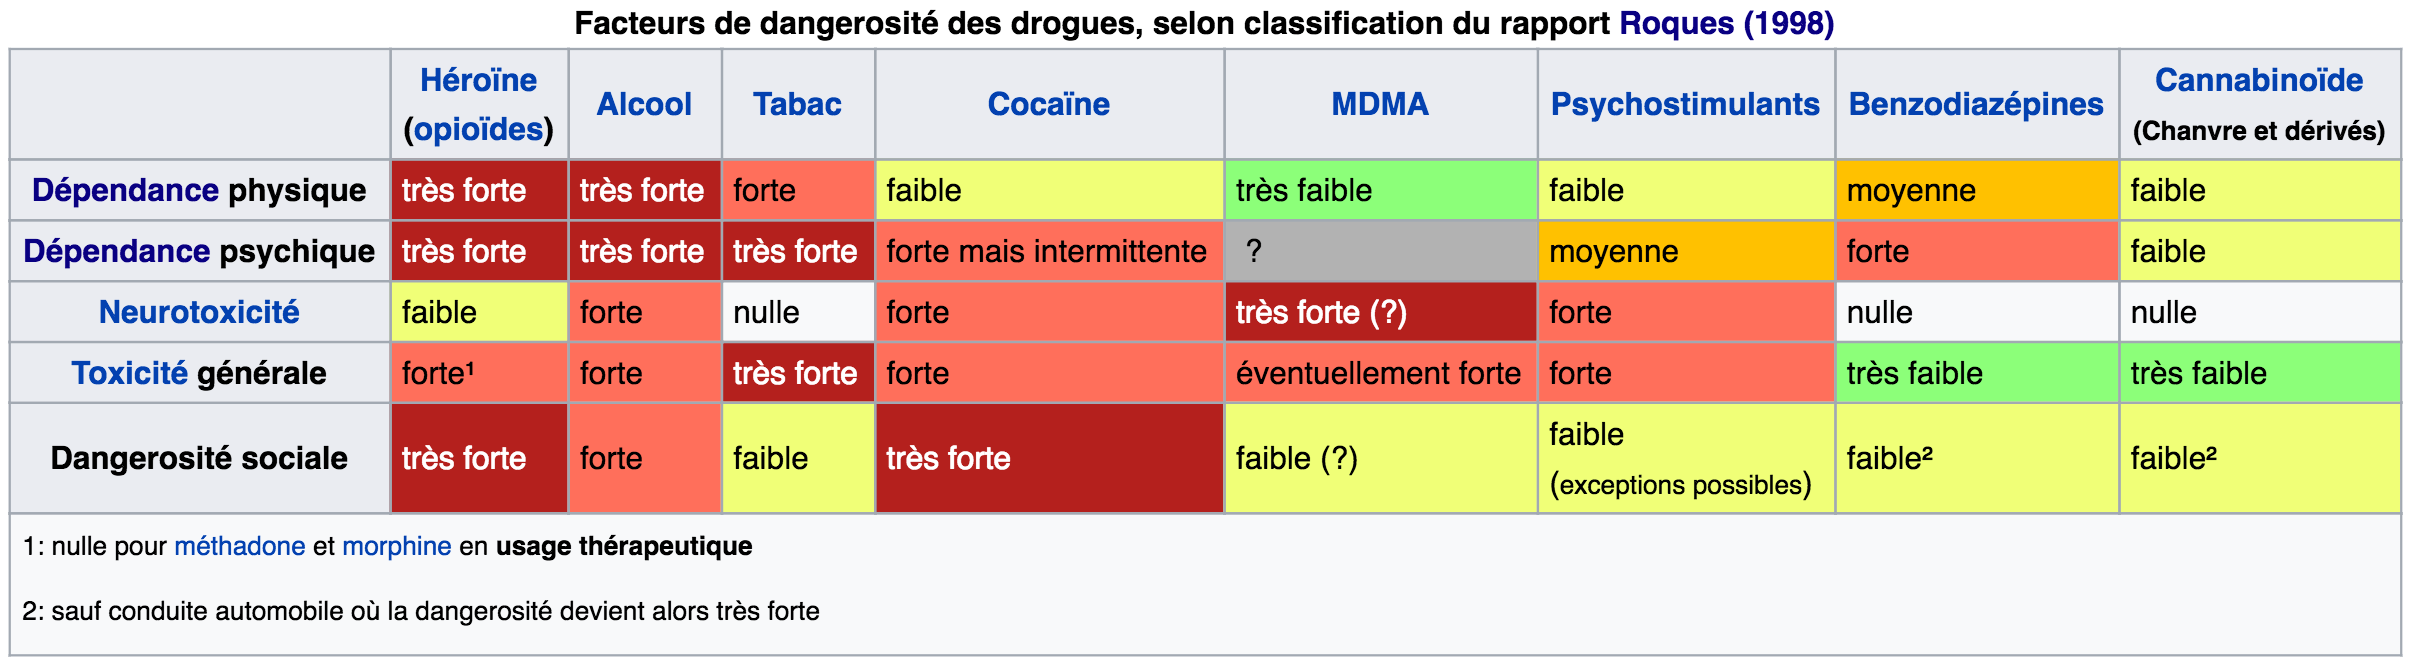
\includegraphics[width=\textwidth]{images/dependance.png}
    \caption{Comparaison des impacts sur la santé de différentes drogues}
    \label{tab:drogues}
\end{table}

   
Cependant selon Amine Benyamina, addictologue et président de la fédération française d’addictologie, il y a un réel danger liant le cannabis et la santé publique, qui concerne l’existence d’une population à risque. Cette population est constituée de deux groupes pour lesquels la consommation de cannabis est néfaste. Le premier est les jeunes, chez qui la  consommation peut nuire à la croissance du cerveau qui n’est pas encore achevée. Le second est constitué des personnes souffrant de troubles psychiatriques, dont un exemple souvent cité est celui de la schizophrénie. Le cannabis n’est pas responsable de cette maladie, en effet on peut remarquer que depuis plusieurs années la consommation de cannabis augmente tandis que le nombre de schizophrène reste lui constant, cependant il peut être responsable du déclenchement de la maladie chez les schizophrènes latents. \cite{franceCulture}).  Il est en même temps intéressant de savoir que le cannabis peut être utilisé comme anti-psychotique dans le traitement alternatif de certaines maladies psychotiques.   

\paragraph{Les bienfaits du cannabis :}

Nous pouvons donc maintenant nous demander quels sont les bienfaits du cannabis. Depuis plusieurs milliers d’années le cannabis est exploité pour nombre de ses caractéristiques (d’ailleurs, aux USA, la première loi qui a été faite sur le cannabis obligeait les fermiers à cultiver du chanvre).  Le chanvre est en effet une fibre très robuste et durable, il permet la fabrication de tissu, d’huile, de papier, et notamment, et c’est ce qui nous intéresse ici, la création de remèdes. Le cannabis a différentes propriétés médicinales : 
\begin{description}
	\item[Analgésiques] malades en phase terminale et pour les douleurs chroniques résistantes aux traitements traditionnels ; 
    \item[Relaxantes et somnifères] malades en phase terminale, troubles du sommeil ; 
    \item[Anti-spasmodiques] sclérose en plaques, épilepsie ; 
    \item[Anti-vomitives] traitement des effets secondaires de la chimiothérapie ou d'autres traitements lourds ;
    \item[Stimulant l'appétit et redonnant l'envie de manger] lutte contre la cachexie (maigreur extrême) et favorise la prise de poids ; 
    \item[Broncho-dilatatrices] asthme ; 
    \item[Anti-inflammatoires] le cannabidiol CBD non psychoactif est connu pour ses affinités avec les récepteurs CB2 situés sur les cellules immunitaires T;
    \item[Anti-psychotiques] traitement alternatif de la schizophrénie ; 	\item[Anti-dépresseur ;] 
    \item[Anxiolytiques ;]
    \item[Sédatives ;] 
    \item[Vasodilatatrices] glaucome, migraines ; 
    \item[Orexigènes] stimulation de l'appétit, en cas de maigreur importante ou de cachexie chez personnes âgées en long séjour, les patients atteint d'une maladie d'Alzheimer ou du sida ; 
    \item[Antalgiques] dans les cas de névralgie. 
\end{description}

Ses avantages naturels sont donc nombreux et intéressants pour la médecine, mais seul quelques médicaments à base de THC sont aujourd’hui présents sur le marché en France \cite{wikicannabismedical}. Pourtant ces remèdes à base de cannabis présentent de nombreux avantages : en plus d’être efficaces, ils sont ce qui se fait de plus naturel et ils sont surtout accessible à quiconque sait entretenir une plante. Une question se pose alors, pourquoi ces médicaments ne sont pas plus répandus? 

\paragraph{Le cannabis et ses mystères :}

Pourquoi la France garde-t-elle des réticences face à l’idée de laisser le chanvre libre sur son territoire sachant qu’à côté de cela elle n’en a aucune à être le troisième producteur mondial de morphine ? La France produit en effet 20\% du pavot légalement cultivé dans le monde, plante utilisé dans la médecine sous la forme de morphine mais aussi dans le milieu de la drogue sous l’appellation d’héroïne. Y a-t-il des enjeux derrière le sujet du cannabis ? 
